\chapter{Aplikacja rozwiązująca problem przydziału kwadratowego z wykorzystaniem kwantowego algorytmu ewolucyjnego}
\label{cha:aplikacja}
Jednym z celów realizowanej pracy dyplomowej było napisanie aplikacji, która przy wykorzystaniu jednego z algorytmów aproksymacyjnych będzie rozwiązywać problem przydziału kwadratowego. Wybór padł na kwantowy algorytm ewolucyjny NPQGA opisany w rozdziale czwartym. Uwzględnione w nim zmiany oraz modyfikacje zostały przedstawione w piątym rozdziale. Program został zrealizowany jako aplikacja konsolowa i napisany w języku C\#.

\section{Interfejsy klas}
Punktem wyjścia do rozpoczęcia prac był zestaw interfejsów klas przygotowanych przez opiekuna niniejszej pracy. Interfejs klasy w sensie języka C\# jest narzędziem wykorzystywanym w technice dziedziczenia i określa metody i właściwości, jakie klasa dziedzicząca po nim musi implementować. Jednakże ciała metod nie są określone i zależą wyłącznie od implementacji w danej klasie. W przeciwieństwie do dziedziczeniu po klasach, istnieje możliwość dziedziczenia po wielu interfejsach. Dzięki wykorzystaniu interfejsów, napisane na potrzeby pracy klasy będzie można wykorzystać w innych aplikacjach :już istniejących, ale i w tych, które dopiero powstaną. Poniżej znajduje się lista interfejsów, które należało zaimplementować:
\begin{enumerate}
\item IEvolutionAlgorithm,
\item IOptimisationAlgorithm,
\item IPopulation,
\item ISolution,
\item IEvolutionaryOperator,
\item IMutationOperator,
\item ICrossoverOperator.
\end{enumerate}

Interfejs \textit{IEvolutionAlgorithm} dziedziczy po interfejsie \textit{IOptimisationAlgorithm}. Na bazie tych interfejsów powstała klasa \textit{QgAlgorithm} zawierająca metody pozwalające na ustawienie i uruchomienie algorytmu oraz pozwalająca na zwrócenie rezultatów działania algorytmu.

Interfejsy \textit{ICrossoverOperator} i \textit{IMutationOperator} dziedziczące po interfejsie \textit{IEvolutionaryOperator} posłużyły jako podstawa, dla stworzenia klas realizujących zadania operatorów krzyżowania oraz mutacji. Na podstawie interfejsu \textit{ICrossoverOperator} powstała również klasa reprezentująca operator bramki kwantowej.

Interfejsy \textit{IPopulation} i \textit{ISolution} posłużyły do napisania klas reprezentujących odpowiednio pojedyncze rozwiązanie algorytmu i populację algorytmu.

\section{Struktura danych}
By algorytm mógł znaleźć rozwiązanie problemu, musi przetwarzać całą populację rozwiązań. Dlatego też została napisana klasa \textit{Population}, dziedzicząca po interfejsie \textit{IPopulation}. Populacja natomiast zawiera w sobie listę osobników, rozwiązań, które reprezentowane są przez obiekty klasy \textit{Solution} dziedziczącej z kolei po interfejsie \textit{ISolution}. Postacią rozwiązania w problemie przydziału kwadratowego jest permutacja, określająca, który obiekt został przypisany do kolejnych lokalizacji. Z tego powodu obiekty klasy \textit{Solution} zawierają w sobie listę obiektów reprezentujących elementy permutacji. Klasa tych obiektów została nazwana \textit{Chromosome}. Należy tutaj wyjaśnić pewną nieścisłość w terminach używanych w algorytmach genetycznych. \textit{Chromosomami} zwykło się nazywać kompletne rozwiązania, a ich fragmenty kodujące rozwiązanie \textit{genami}. Z racji, iż w aplikacji rozwiązania problemu reprezentowane są przez obiekty klasy \textit{Solution}, a element permutacji nie jest najmniejsza porcją informacji, postanowiono nazwać te porcje chromosomami, a ich najmniejszą część \textit{genem}. A więc \textit{chromosomy} składają się z kubitów reprezentowanych przez klasę \textit{Qbit}. Poprzez zdekodowanie stanu kubitów określa się wartość chromosomu, a następnie poprzez omówioną w rozdziale czwartym konwersję otrzymuje się permutacyjną postać rozwiązania problemu QAP.
\newpage
\begin{figure}[!t]
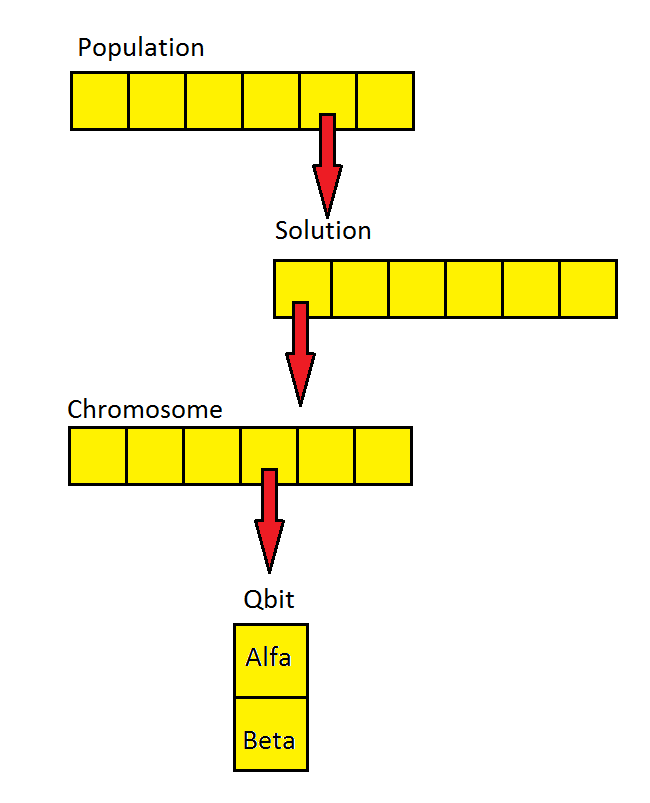
\includegraphics[scale=0.4]{data_structure}
\caption{Struktura danych}
\end{figure}

W kontekście struktury danych należy jeszcze wspomnieć o macierzach przepływu i odległości problemu QAP. Ich wartości są wczytywane z plików \textit{.dat} zawierających rozmiar problemu oraz odpowiednio macierze odległości i przepływu i są następnie trzymane w obiekcie klasy \textit{QapData} zrealizowanej jako singleton, czyli jako specjalna klasa o globalnym dostępnie pozwalająca na utworzenie tylko jednego jej obiektu. Posiada ona także mechanizmy, które bez wiedzy użytkownika same dbają o to, by faktycznie istniał jeden jej obiekt i jej instancja została utworzona podczas pierwszej próby jej użycia.

\section{Funkcja testująca działanie algorytmu}
Oprócz klas związanych z samym algorytmem NPQGA, została napisana klasa pozwalająca na przetestowanie algorytmu. Składa się ona z dwóch funkcji: testującej oraz wczytującej instancje problemu QAP i zapisującej wartości macierzy przepływu i odległości do opisanego wyżej singletona.

Po wywołaniu funkcji testującej algorytm użytkownik proszony jest o podanie dla ilu wartość testowanego parametru chce przeprowadzić testy oraz ile razy powtórzyć eksperyment dla danej wartości parametru. Następnie należy podać, który parametr algorytmu (operator selekcji, operator krzyżowania, prawdopodobieństwo krzyżowania, prawdopodobieństwo mutacji, operator bramki kwantowej) ma być testowany. Po tym wyborze użytkownik proszony jest o podanie kolejnych wartości wybranego parametru algorytmu. Kolejnym krokiem jest wybór instancji testowych, dla których mają zostać przeprowadzone eksperymenty, a następnie należy ustawić pozostałe parametry algorytmu, których wartość będzie stała podczas wszystkich testów. Ostatnim krokiem jest podanie szablonu nazwy pliku, do którego zostaną zapisane rezultaty testów. 

W przypadku operatora selekcji do wyboru są dwie metody: ruletkowa oraz rankingowa. Spośród metod krzyżowania dostępne są trzy opcje: CX, OX i PMX. Wersje bramki kwantowej zostały opisane w rozdziałach 4 i 5. Istnieje także możliwość uruchomienia algorytmu bez bramki kwantowej.

W obrębie testowania różnych wartości jednego parametru dla jednej instancji testowej populacja startowa generowana jest raz i służy jako punkt wyjścia dla każdego z testów.

Aplikacja została napisana w sposób niepozwalający na przyjęcie nieprawidłowych danych.

Po zakończeniu testów użytkownik ma możliwość ponownego rozpoczęcia eksperymentów lub zamknięcia aplikacji.

\section{Rezultaty działania aplikacji}
Wyniki działania eksperymentów zapisywane są w pliku \textit{xls} bądź \textit{xlsx}, w zależności od wersji oprogramowania \textit{Microsoft Excel} zainstalowanej na komputerze użytkownika aplikacji. Dla każdej z wybranych instancji testowych tworzony jest osobny plik o nazwie w formacie [szablon nazwy]\_[parametr testowany]. W osobnych arkuszach danego pliku znajdują się rezultaty testów dla poszczególnych wartości testowanego parametru.

Na rezultaty eksperymentów składają się następujące wartości:
\begin{itemize}
\item wartość funkcji celu najlepszego rozwiązania z populacji startowej,
\item wartość funkcji celu najlepszego rozwiązania znalezionego podczas wszystkich przeprowadzonych testów dla danej wartości testowanego parametru,
\item średnia wartość najlepszych rozwiązań zwróconych przez algorytm w powyższych testach,
\item numer iteracji, w której najlepsze rozwiązanie zostało znalezione,
\item średnia wartość numerów iteracji najlepszych rozwiązań w poszczególnych testach.  
\end{itemize}

\section{Szczegóły związane z implementacją poszczególnych elementów algorytmu}
Kilka szczegółów związanych z działaniem algorytmu nie zostało poruszonych w publikacji \cite{NPQGA}. Jednakże, by algorytm mógł działać, należało arbitralnie przyjąć pewne założenia. Jednym z takich założeń jest moment aktualizacji stanu kubitów. Zostało przyjęte, że należy ocenić, w którym ze stanów 1 lub 0 znajduje się bit kwantowy, gdy wiadome jest, że rozwiązanie, w którym dany kubit się znajduje, poddane zostało zmianom wynikającym z działania operatora bramki kwantowej, lub dla tego rozwiązania zostały spełnione warunki na zajście mutacji. Natomiast po dokonaniu operacji krzyżowania, nie jest oceniany stan kubitów rozwiązań potomnych. Taka ocena, szczególnie w początkowych iteracjach algorytmu powodowałaby, że rozwiązania otrzymane na drodze krzyżowania mogłyby tracić informację uzyskaną z rozwiązań rodziców. Ideą krzyżowania jest wymiana informacji.

W przypadku, gdy użytkownik programu postanowi, że algorytm ma znajdywać rozwiązanie bez wykorzystania bramki kwantowej, kwantowa idea algorytmu przejawia się wtedy jedynie podczas tworzenia populacji początkowej oraz operacji mutacji, która dalej polega na zamianie wartości parametrów $\alpha$ i $\beta$.

Rozwiązanie, które jest podstawą do działania bramki kwantowej i nazywane jest najlepszym, jest faktycznie najlepszym rozwiązaniem, ale uzyskanym w poprzednim pokoleniu. Operator bramki kwantowej używany jest dopiero na populacji poddanej już działaniu operatorów krzyżowania i mutacji. Z tego powodu istnieje możliwość, że dopasowanie zapamiętanego rozwiązania będzie gorsze niż dopasowanie niektórych rozwiązań poddawanych działaniu bramki kwantowej. Wynika to z faktu, iż w efekcie działania operatorów mutacji i krzyżowania mogą powstać rozwiązania lepsze niż te, które dotychczas istniały w populacji. Dlatego rozważane są w tablicach \textit{Look Up} przypadki, dla których warunek $f(x)>f(best)$ może być prawdą.

Foldery z rezultatami działania algorytmu - \textit{Results} i instancjami testowymi - \textit{QAPLib} znajdują się w tym samym folderze co plik wykonywalny aplikacji. Podczas uruchamiania funkcji testującej sprawdzane jest na początku czy wymienione foldery istnieją. Jeśli nie, są tworzone i użytkownik jest o tym powiadamiany. Następnie funkcja kończy swoje działanie.

Próba uruchomienia testów, gdy folder z instancjami jest pusty, gdy nie udało się odczytać danych z pliku z danymi dla problemu QAP bądź nastąpił błąd podczas zapisu danych do pliku z rezultatami działania algorytmu, zgłaszany jest błąd, po czym funkcja kończy swoje działanie.